% REVISÃO DE LITERATURA--------------------------------------------------------

\chapter{REVISÃO BIBLIOGRÁFICA}
\label{chap:fundamentacaoTeorica}

\section{Turbinas hidrocinéticas}

A potencia gerada por uma turbina pode ser expressa pela \autoref{eq:Power}.

\begin{equation}
P = \frac{1}{2}A\rho {V^3}{C_P}
\label{eq:Power}
\end{equation}

Sendo $A$ a área do rotor da turbina ($m^2$), $\rho$ a massa específica do fluido ($kg/{m}^3$), $V$ é a velocidade de corrente ($m/s$) e $C_P$ o coeficiente de potência (adimensional). O coeficiente de potência de uma turbina hidrocinética indica a quantidade de energia mecânica extraída a partir da energia disponível no fluido. A máxima eficiência que uma turbina hidrocinética ideal pode alcançar é dada pelo Limite de Betz-Joukowski que corresponde a 59,3\%, o equivalente a um $C_P$ de 0,593 \cite{vallverdu2014, SHINOMIYA2015d}.

\subsection{Princípios de funcionamento, classificação e principais componentes}

A \autoref{fig:Behrouzi2014-2} apresenta algumas configurações possíveis.

\begin{figure}
	\centering
	\begin{subfigure}{0.31\textwidth}
		\centering
		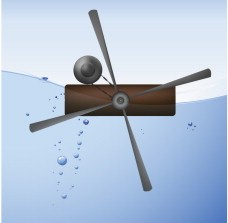
\includegraphics[scale=0.9]{figuras/VermaakVa.jpg}
		\caption{Eixo no plano.}
		\label{subfig:Inplane}
	\end{subfigure}
	\begin{subfigure}{0.31\textwidth}
		\centering
		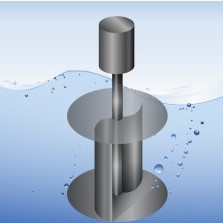
\includegraphics[scale=0.9]{figuras/VermaakVf.jpg}
		\caption{Savonius.}
		\label{subfig:Savonius}
	\end{subfigure}
	\begin{subfigure}{0.31\textwidth}
		\centering
		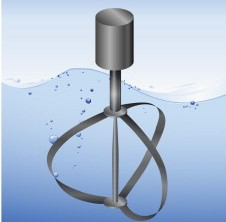
\includegraphics[scale=0.9]{figuras/VermaakVd.jpg}
		\caption{Darrieus.}
		\label{subfig:Darrieus}
	\end{subfigure}
	\begin{subfigure}{0.31\textwidth}
		\centering
		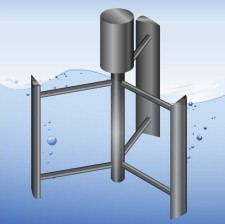
\includegraphics[scale=0.9]{figuras/VermaakVc.jpg}
		\caption{Darrieus - H.}
		\label{subfig:DarrieusH}
	\end{subfigure}	
	\begin{subfigure}{0.31\textwidth}
		\centering
		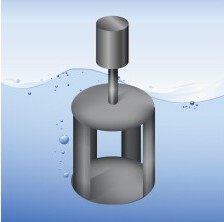
\includegraphics[scale=0.9]{figuras/VermaakVb.jpg}
		\caption{Darrieus gaiola de esquilo.}
		\label{subfig:SquirrelcageDarrieus}
	\end{subfigure}
	\begin{subfigure}{0.31\textwidth}
		\centering
		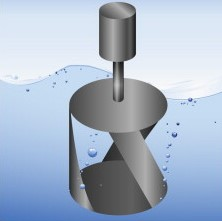
\includegraphics[scale=0.9]{figuras/VermaakVe.jpg}
		\caption{Gorlov.}
		\label{subfig:Gorlov}
	\end{subfigure}	
	\caption{Turbinas hidrocinéticas de eixo vertical.}
	\fonte{\citeonline{harris2006essential}.}
	\label{fig:Behrouzi2014-2}
\end{figure}

\subsection{Modelos de predição de performance hidrodinâmica}

Uma revisão sobre modelos de predição de performance para turbinas eólicas de eixo vertical incluem os trabalhos de \citeonline{Brahimi1995}, \citeonline{paraschivoiu2002prediction}, \citeonline{paraschivoiu2002wind} e \citeonline{ISLAM20081087},  que serviram como ponto de partida para os modelos hidrodinâmicos \cite{Dai2011}. 
